\documentclass[../thesis.tex]{subfiles}
\graphicspath{{\subfix{figs/ses_ling/}}}
\addbibresource{biblio.bib}
\begin{document}

\chapter{Socio-economic boundaries and standard language}
\label{ch:ses_ling}

\epigraph{
  This was not to say that Albertine had not already possessed [...] a quite
  adequate assortment  of those expressions which reveal at once that one's people are
  in easy circumstances, and which, year by year, a mother passes on to her daughter
  just as she bestows on her [...]
  %, gradually, as the girl grows up, on important occasions,
  her own jewels.
}{
  \epigraphcite{ProustGuermantesWay1927}
}

Language bounds individuals together just as much as it divides them. Upon reading the
last sentence, one may first think of interlanguage boundaries as the ones we have seen
in the previous chapter: if two individuals cannot understand each other's language,
communication is effectively very limited. This chapter, on the other hand, is dedicated
to intra-language differences: when people speak the same language, but differently,
which is also a strong marker of social divides. As we already emphasized in
\cref{ch:origins_lang_diversity}, language variation in a population is driven by many
factors, among which the socio-economic background of individuals is essential. And as
we also said previously, one's ability to use the standard form of their language can be
associated to a higher linguistic capital, and has thus economic values. It is not
uncommon that some classes of the population, particularly those of relatively low
\ac{SES}, prefer to use the non-standard form. This has been shown by prominent
sociolinguists in the past, as they conducted field studies and analysed differences
between socio-economic classes
\cite{LabovSocialStratification1966,TrudgillSocialDifferentiation1974}. Although this
phenomenon has long been known \cite{ChambersSociolinguisticTheory2007}, it has been
observed on very limited scales, and, more importantly, no real explanation of how it
might emerge has been proposed. These are the two shortcomings we wish to address in
this chapter. As groups of lower \ac{SES} have less linguistic capital, their economic
opportunities will also be affected. \Ac{SES} and this linguistic variation are thus
mutually sustaining: one inherits a \ac{SES} along which comes a linguistic capital that
contributes --- among other things --- to constrain them to their status of origin.
Understanding the mechanisms that lead to this linguistic segregation is therefore of
great importance. 

First, as we have already shown in previous chapters, a first step toward understanding
is to measure the phenomenon. It has already been quantified by the PISA reports of the
OECD \cite{OECDWhereAll2019}, which consistently show that students with lower
socio-economic background tend to have a lower reading proficiency. While these confirm
there is an issue to tackle, they are not extensive enough. They do not test language
production, and not the whole population but only a sample of students of a specific
age. Alternative empirical works are thus needed. Data from social media have repeatedly
proven useful to link \ac{SES} and different social behaviours
\cite{GaoComputationalSocioeconomics2019}. In particular, Twitter data were used in the
past to study geographical variation of linguistic variables
\cite{EisensteinDiffusionLexical2014}. Closer to our topic of interest still, some past
work has investigated the dependence on \ac{SES} of the frequency of a few markers of
non-standard language in France, as seen on Twitter
\cite{AbitbolSocioeconomicDependencies2018}, showing the potential of this data source
for such an analysis. Here, we investigate these dependencies in England and Wales, by way of
measuring how Twitter users abide by the rules of the standard variety of their
language.


% \cite{LaksWhyThere2013} In such a conception, communication is a leading force in the emergence and stabilization of human linguistic competence, both diachronically and synchronically. In this approach, variation and heterogeneity are to be seen as core factors in shaping language. Thus, as argued some 50 years ago by Weinreich, variation and heterogeneity are to be regarded as structurally functional, and as fundamental dimensions of language.
% \cite{KinzlerNativeLanguage2007} social groups are partly built and opposed based on language, and very early

\section{An influence of socio-economic status?}

\subsection{Twitter data analysis}
To do so, we analyse the tweets written in English by users identified as UK residents,
following the methodology described in \cref{sec:methods_twitter}. To assign a \ac{SES}
to these users, we also determine their area of residence from the geotags attached to
their tweets. Our unit areas for the study are the \SI{7201}{} \acp{MSOA}, which are
areas created by the Office for National Statistics of the UK for the output of the
census estimates. They host at least \SI{5000}{} and at most \SI{15000}{} inhabitants,
with a typical population of \SI{10000}{}. Their boundaries can be downloaded from the
Open Geography portal of the Office for National
Statistics\footnote{\url{https://geoportal.statistics.gov.uk/maps/msoa-dec-2011-boundaries-generalised-clipped-bgc-ew-v3}}.
Importantly, the average annual net income of their residents can be obtained from the
census\footnote{In particular the 2018 net annual income estimates, available at
\url{https://www.ons.gov.uk/employmentandlabourmarket/peopleinwork/earningsandworkinghours/datasets/smallareaincomeestimatesformiddlelayersuperoutputareasenglandandwales}},
which gives us a proxy for the \ac{SES} of our Twitter users.

The second ingredient we need for our analysis is their propensity to deviate from the
rules defining standard English. The solution we picked to measure these deviations is
LanguageTool, an open-source grammar, style and spell checker. The first advantage of
using such a tool over a pre-defined set of rules, as in
\cite{AbitbolSocioeconomicDependencies2018}, is that the tool is implemented in 15
languages. Our study can thus quite easily be replicated in other countries. The second
advantage is that it covers a very wide spectrum of potential mistakes: it has more than
\SI{5500}{} rules defined for the English language. These rules are categorised in 11
categories, among which are grammar mistakes, confused words or typos. In this work we
focus on grammar mistakes, as they are among the most common and are the most
characteristic of non-standard language. LanguageTool therefore enables us to compute
the frequency at which Twitter users identified as UK residents make grammar mistakes,
according to standard rules. From this raw frequency we then compute the frequency of
mistakes per word written by the user. As in the previous chapter, we compute this
frequency on a user level, to try and be more representative of the general population,
and not only of the few, very active users. At the cell level, we then compute the
average of these relative frequencies for all residents. This implies that we cannot
keep all users, as some have been so little active that they did not write enough to
make mistakes, so we keep only users who have written at least 100 words. Also, to
exclude cells with too little statistics, in the following we only keep cells with at
least 15 residents left after this previous filter. This leaves us with \SI{131402}{}
users spread across \SI{4879}{} \acp{MSOA}. In each of these cells, our analysis yields
an estimate of the income of its residents and of the frequency at which they make
grammar mistakes.


\subsection{Correlations with the frequency of mistakes}
We find a significant, but weak correlation (Pearson r equal to -0.25) between the net
income and the average frequency of mistakes in all cells of the country. We then focus
on metropolitan areas because we expect them to host more linguistic and socio-economic
heterogeneity than their rural counterparts. We also happen to have more data in these
on both mobility and language production, due to the fact that Twitter users tend to be
more urban \cite{MisloveUnderstandingDemographics2011}. We therefore consider the 8
largest metropolitan areas in England, and find large differences between these areas,
with correlations ranging from -0.07 in Sheffield to -0.5 in Bristol. The average
frequency of grammar mistakes is plotted against the average of net annual income of
their residents for all \acp{MSOA} of England and Wales, London, Manchester and
Sheffield in \cref{fig:ses_x_grammar_corrs}.
\begin{figure}
\centering
  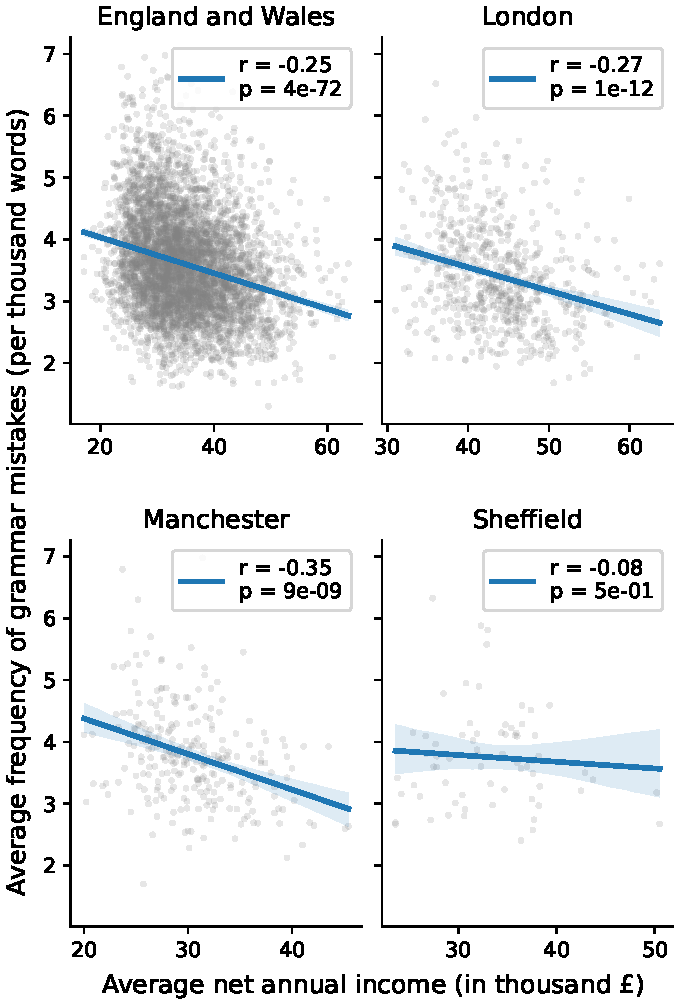
\includegraphics[width=\textwidth]{ses_x_grammar_corrs}
  \caption{ Correlation between frequency of grammar mistakes and net income. We show
  them for all \acp{MSOA} of England and Wales, and then of the metropolitan areas of
  London, Manchester and Sheffield. Each grey dot corresponds to an \ac{MSOA}, while
  blue lines indicate the result of a linear regression, with the corresponding Pearson
  r and p-value given in each legend. The areas coloured in light blue indicate the
  \SI{95}{\percent} confidence interval for the regression estimates.}
  \label{fig:ses_x_grammar_corrs}
\end{figure}


\subsection{The role of assortativity}
% \cite{EagleNetworkDiversity2010} We find that the diversity of individuals’
% relationships is strongly correlated with the economic development of communities.
% hence why we turn to measuring social mixing next. hein??

To find out what could make these cities so different in that regard, we measure the
assortativity in the mobility patterns of their residents
\cite{HilmanSocioeconomicBiases2022}. We thus determine how likely people from different
socio-economic classes are to interact with each other.

\Ac{SES} classes are defined such that each class has roughly the same population. Since
our proxy for \ac{SES} is the average income in every \ac{MSOA}, every resident of a
cell will necessarily be assigned to the same class. Considering the cells in a given
metropolitan area, we rank them by increasing average net income. We get their
population from the
census\footnote{\url{https://www.nomisweb.co.uk/census/2011/ks101uk}}, denoted $N_c$ for
each cell $c$ in the following. Denoting $P_c$ the set of cells less populated than $c$,
formally defined as $P_c = \left\{ c' \in C \mid N_{c'} < N_c \right\}$, we define the
\ac{SES} class of $c$ as follows:
\begin{equation}
  S_c = n_S \left\lceil \frac{\sum_{c' \in P_c} N_{c'}}{\sum_{c' \in C} N_{c'}} \right\rceil,
\end{equation}
with $\left\lceil \cdot \right\rceil$ representing the ceiling function and $n_S$ the
number of classes we wish to define. We denote $t_{u, c}$ the number of trips made by
user $u$ to cell $c$, and introduce the probability for an individual residing in a cell
of class $i$ to visit another of class $j$:
\begin{equation}
  \label{eq:class_visit_proba}
  M_{i, j} = \frac{
      \sum_{u \in S_i} \sum_{c \in S_j} t_{u, c}
    }{
      \sum_{j \in S_j} \sum_{u \in S_i} \sum_{c \in S_j} t_{u, c}
    },
\end{equation}
which is normalised row-wise, meaning $\sum_j M_{i, j} = 1$. Since we are interested in
how much individuals mix when they move, we exclude the tweets sent from their cell of
residence to compute $M_{i, j}$. Such matrices computed for our eight metropolitan areas
are represented in \cref{fig:cities_SES_mobility}. They show completely different
patterns, from cities where the diagonal elements slightly stand out as in London or
Manchester, to cities in which one specific class of cells is the destination of most
outward mobility, as in Newcastle or Bristol.
\begin{figure}
\centering
  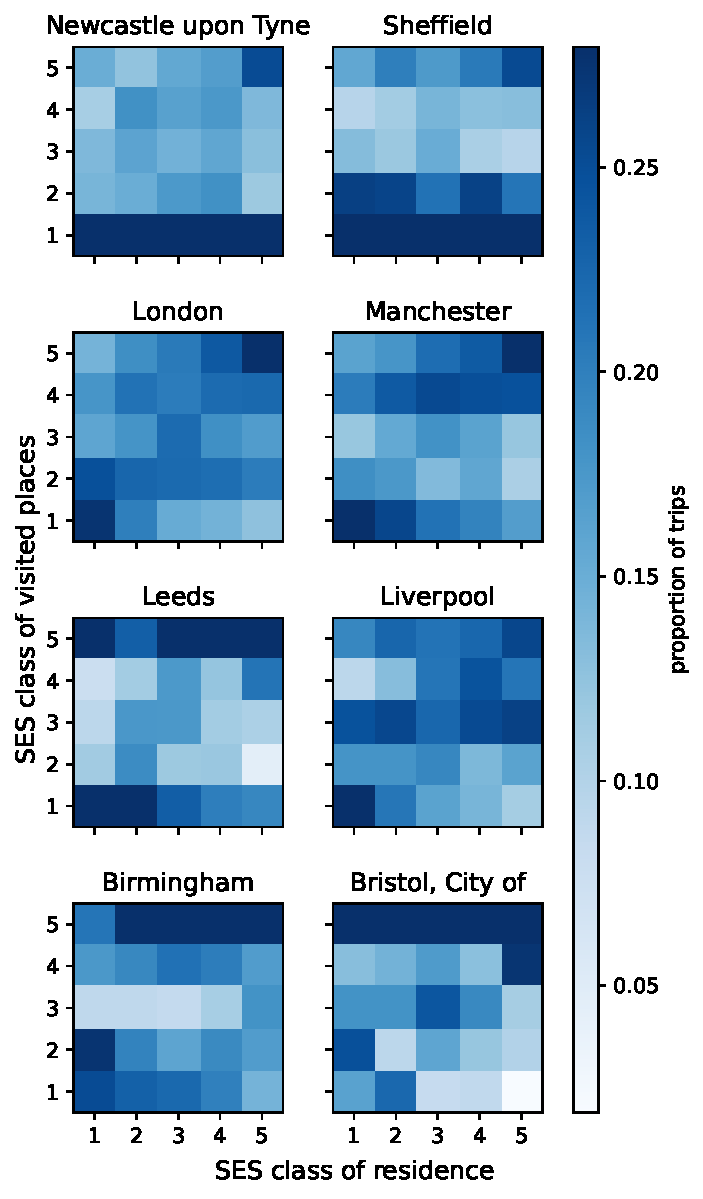
\includegraphics[width=0.9\textwidth]{cities_SES_mobility}
  \caption{ Matrices of stratification of \ac{SES} classes in their mobility in eight
  metropolitan areas of England. For every pair of \ac{SES} classes for the cell of
  residence and the cell visited by Twitter users, this shows the proportion of trips
  that were made from the latter to the former. A square located at $(x, y) = (i, j)$
  corresponds to $M_{j, i}$, as it is defined in \cref{eq:class_visit_proba}. The
  normalisation is thus column-wise on this representation.}
  \label{fig:cities_SES_mobility}
\end{figure}

These patterns can be summarised by a measure of how strongly diagonal these matrices
are: their Pearson r value, denoted $r_M$ in our case. It is defined as follows:
\begin{equation}
  r_M = \frac{
      \sum_{i, j} M_{i, j} \cdot \sum_{i, j} i j M_{i, j}
      - \sum_{i, j} i M_{i, j} \cdot \sum_{i, j} j M_{i, j}
    }{
      \sqrt{\sum_{i, j} i^2 M_{i, j} - \left( \sum_{i, j} i M_{i, j} \right)^2}
      \cdot \sqrt{\sum_{i, j} j^2 M_{i, j} - \left( \sum_{i, j} j M_{i, j} \right)^2}
    }.
\end{equation}
This gives us a measure of assortativity, meaning that this metric gives us a sense of
how much people of similar classes tend to stay together. The closer to 1, the more
individuals tend to go to areas of similar \ac{SES} (assortative mixing), and the closer
to -1, the more they will stay with people of opposite \ac{SES} (disassortative mixing).
Values close to 0 indicate no assortativity, meaning no preference in mixing. We measure
this assortativity for our metropolitan areas from the matrices shown in
\cref{fig:cities_SES_mobility}, and show the results in
\cref{fig:cities_assort_vs_grammar_and_SES_corr} against the correlation we computed
previously between socio-economic status and the average frequency of grammar mistakes.
What we find is a very clear correlation between this assortativity measured at the city
level, and the correlation between \ac{SES} and the frequency of grammar mistakes. This
indicates that the more mixing in the population, the less the frequency of mistakes is
determined by the \ac{SES} of origin. Further, as shown in the bottom panel of
\cref{fig:cities_assort_vs_grammar_and_SES_corr}, more mixing tends to imply more
frequent mistakes. It then appears to favour the spread in popularity of non-standard
English.
\begin{figure}
\centering
  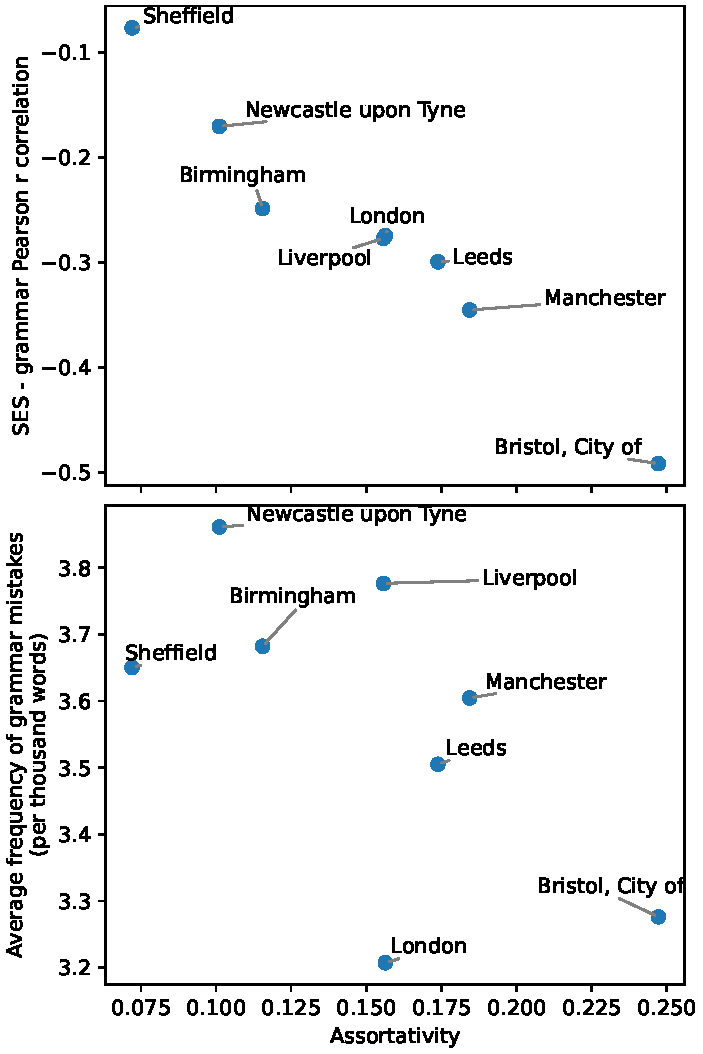
\includegraphics[width=0.9\textwidth]{cities_assort_vs_grammar_and_SES_corr}
  \caption{The influence of assortativity on the frequency of grammar mistakes (bottom)
  and their dependence on \ac{SES} of origin (top). The latter clearly decreases as
  assortativity increases. This means that the more \ac{SES} classes mix with one
  another, the less the usage of the standard form of individuals will depend on their
  own \ac{SES}. As for the frequency of mistakes, it seems to rather increase with
  mixing.}
  \label{fig:cities_assort_vs_grammar_and_SES_corr}
\end{figure}



\section{Model}

\subsection{Definition}
Having identified the importance of social mixing, we wish to understand the mechanisms
behind this observation with a simple model.
% There are models for cultural transmission, like the literature centered around the
% Axelrod model
% \cite{AxelrodDisseminationCulture1997,CastellanoNonequilibriumPhase2000,KlemmGlobalCulture2003,KlemmNonequilibriumTransitions2003,BattistonLayeredSocial2017}.
% No dependence on intrinsic attribute, or group identity, have been taken into account.
% Cultural traits like the use of a language variety can depend on an individual sense of
% identity.
There are several effects we wish to
consider, that we describe below.
\begin{enumerate}[(i)]
  \item One of the two varieties of the language may be more prestigious than the other.
  This is for example the case of the standard form: it is taught at schools and spoken
  by mainstream media and public institutions \cite{DavilaInevitabilityStandard2016}.
  \item Even though one variety is less prestigious, it might still be preferred by a
  part of the population that has some kind of cultural attachment to it. For instance,
  slang can be preferred by members of lower \ac{SES}, as using it might give them a
  sense of group identity
  \cite{LabovSocialStratification1966,TrudgillSocialDifferentiation1974}.
  \item We previously observed very different mixing patterns in English metropolises.
  Indeed, mobility can be very heterogeneous, so it should be possible to plug in any
  mobility pattern into the model to be able to understand how different mixing may
  affect the dynamics of the linguistic varieties.
\end{enumerate}
With these considerations in mind, we propose an \ac{ABM}, that we describe next. It
considers agent who can have one of two \ac{SES} classes,
% each class living in one of
% two cells, and
% TODO: keep this way? stay general on number of cells/classes?
who can either speak standard, or not. The standard form has an intrinsic prestige
$l_v$, the value of which belongs to the unit interval, but that we will always set
above 0.5 in the following, to account for (i). Now turning to (ii), each \ac{SES} class
has a preference for one form: the lower class 1 is attached to the non-standard form
with a factor $q_1$, and inversely the higher class 2 is attached to the standard one
with $q_2$. They are also comprised between 0 and 1, and when one of these two
parameters has a value above $0.5$, it means there is a preference for the respective
form. Then for instance, when an agent of low \ac{SES} speaking non-standard interacts
with another agent speaking standard, they have a probability $l_v (1 - q_1)$ to start
using the standard form as well. The agents can move from their residence cell with a
probability $M_{i,j}$ at each step, which thus controls the mixing of the two
populations, as discussed in (iii). A summary diagram of the model is provided in
\cref{fig:model_diagram}.
\begin{figure}
\centering
  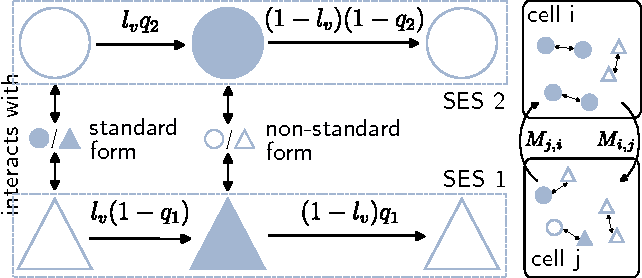
\includegraphics[width=\textwidth]{model_diagram}
  \caption{Diagram summarizing our agent-based model for the adoption of a linguistic
  variety. It features two \ac{SES} classes, represented by circles and triangles, which
  can speak one of two varieties of their language: the standard form (filled shapes)
  and the non-standard (empty shapes). Each agent has a cell of residence, and a
  mobility matrix with elements $M_{i, j}$ defines the probabilities for a resident of
  $i$ to be at different cells at each time step. After they have moved, for every
  agent, another agent is picked randomly for them to interact with, and if they happen
  to interact with an agent using the other variety, in function of their \ac{SES} class
  of origin they have different probabilities to adopt this variety. For instance, when
  a triangle (\ac{SES} 1) speaking non-standard interacts with another agent speaking
  standard, they have a probability equal to $l_v (1 - q_1)$ to adopt the standard form
  (transition represented in the bottom left).}
  \label{fig:model_diagram}
\end{figure}


\subsection{Properties and behaviour in mean-field}
The process we just described above can be simulated for any number of cells and
arrangements of the populations of different \ac{SES} classes. Here, however, we will
consider a rather simple case in order to present succinct equations that lend
themselves to interpretation and mathematical analysis. We will consider only two cells,
with $N_1$ individuals of class 1 residing in cell 1, and $N_2$ individuals of class 2
residing in cell 2. This is a situation of complete socio-economic segregation. We will
denote $p_1$ the proportion of individuals of class 1 speaking non-standard (variety 1),
and $p_2$ the proportion of individuals of class 2 speaking standard (variety 2).
Individuals have to speak either 1 or 2, which implies that. for instance, a proportion
$(1 - p_1)$ of individuals of class 1 speak the variety 2. The two variables therefore
summarise the linguistic state of the system at any given time. Regarding the mobility,
we introduce a new variable $m_{i, j}$, such that:
\begin{equation}
  m_{i, j} \equiv \frac{N_{i} M_{i, j}}{\sum_{i'} N_{s_{i'}} M_{i', j}},
\end{equation}
which can be understood as the probability to pick from $j$ an individual with residence
in $i$. They satisfy $\sum_i m_{i, j} = 1$. Further, since there are only two cells,
people either stay at their residence or move to the other cell. As a result, to account
for different mobility patterns, out of the $2 \times 2$ mobility matrix with elements
$M_{i, j}$, we only retain the parameters $M_1 \equiv M_{1, 2}$ and $M_2 \equiv M_{2,
1}$, the probabilities for people of each class to move away from their residence cell.
Likewise, the matrix of $m_{i, j}$ can be summarised with the corresponding $m_1$ and
$m_2$. Under all these assumptions and new notation, we can then write the probability
to pick an individual speaking a variety in each cell as:
% TODO: ref appendix? include this here?
\begin{equation}
  \left\{
  \begin{aligned}
      P(2 \mid c = c_1)
          = (1 - m_2) (1 - p_1) + m_2 p_2
      \\
      P(2 \mid c = c_2)
          = m_1 (1 - p_1) + (1 - m_1) p_2
      \\
      P(1 \mid c = c_1)
          = (1 - m_2) p_1 + m_2 (1 - p_2)
      \\
      P(1 \mid c = c_2)
          = m_1 p_1 + (1 - m_1) (1 - p_2)
  \end{aligned}
  \right.
\end{equation}
This allows us to write the probabilities to switch from one variant to
another depending on one's \ac{SES} class:
\begin{equation}
  \left\{
  \begin{aligned}
      P(1 \rightarrow 2 \mid s = s_1)
          &= l_v (1 - q_1)
          \begin{aligned}[t]
            &[P(2 \mid c = c_1) (1 - M_1)
            \\
            &+ P(2 \mid c = c_2) M_1]
          \end{aligned}
      \\[1ex]
      P(1 \rightarrow 2 \mid s = s_2)
          &= l_v q_2
          \begin{aligned}[t]
              &[P(2 \mid c = c_1) M_2
              \\
              &+ P(2 \mid c = c_2)(1 - M_2)]
          \end{aligned}
      \\[1ex]
      P(2 \rightarrow 1 \mid s = s_1)
          &= (1 - l_v) q_1
          \begin{aligned}[t]
              &[P(1 \mid c = c_1) (1 - M_1)
              \\
              & + P(1 \mid c = c_2) M_1]
          \end{aligned}
      \\[1ex]
      P(2 \rightarrow 1 \mid s = s_2)
          &= (1 - l_v) (1 - q_2)
          \begin{aligned}[t]
              &[P(1 \mid c = c_1) M_2
              \\
              &+ P(1 \mid c = c_2) (1 - M_2)]
          \end{aligned}
  \end{aligned}
  \right.
\end{equation}
% \begin{equation}
%   \label{eq:final_trans_probs}
%   \begin{aligned}
%       P(1 \rightarrow 2 \mid s = s_1)
%           &= l_v (1 - q_1) [
%             (1 - M_1) P(2 \mid c = c_1)  + M_1 P(2 \mid c = c_2)
%           ]
%       \\
%       P(1 \rightarrow 2 \mid s = s_2)
%           &= l_v q_2 [
%             M_2 P(2 \mid c = c_1) + (1 - M_2) P(2 \mid c = c_2)
%           ]
%       \\
%       P(2 \rightarrow 1 \mid s = s_1)
%           &= (1 - l_v) q_1 [
%             (1 - M_1)P(1 \mid c = c_1) + M_1 P(1 \mid c = c_2)
%             ]
%       \\
%       P(2 \rightarrow 1 \mid s = s_2)
%           &= (1 - l_v) (1 - q_2) [
%             M_2 P(1 \mid c = c_1) + (1 - M_2) P(1 \mid c = c_2)
%           ]
%   \end{aligned}
% \end{equation}
Working in mean field, we can write the following system of differential equations:
\begin{equation}
    \label{eq:ses_ling_time_evol}
    \left\{
    \begin{aligned}
        % v and c depend on t
        \dv{p_1}{t} 
            &= (1 - p_1) P(2 \rightarrow 1 \mid s = s_1)
                - p_1 P(1 \rightarrow 2 \mid s = s_1)
        \\
        \dv{p_2}{t} 
            &= (1 - p_2) P(1 \rightarrow 2 \mid s = s_2)
                 - p_2 P(2 \rightarrow 1 \mid s = s_2)
    \end{aligned}
    \right.
\end{equation}

Now if we simplify further and assume that the two \ac{SES} classes have the same
population, and the same mobility $M = M_1 = M_2$, then we get that $m_1 = m_2 = M$, and
it follows that
\begin{equation}
  \label{eq:ses_ling_time_evol_eq_mob}
  \left\{
  \begin{aligned}
      % v and c depend on t
      \dv{p_1}{t} 
          &=
            % \eqnmarkbox[NavyBlue]{mob1}{
            2 M (1 - M) (1 - p_1 - p_2) [q_1 (1 - l_v) - p_1 (q_1 - l_v)]
          % }
      \\
          & \quad +
          % \eqnmarkbox[OliveGreen]{g1}{
            p_1 (1 - p_1) (q_1 - l_v)
          % }
      \\[1ex]
      \dv{p_2}{t} 
          &=
            % \eqnmarkbox[NavyBlue]{mob2}{
            2 M (1 - M) (1 - p_1 - p_2) [q_2 l_v - p_2 (l_v + q_2 - 1)]
          % }
      \\
          & \quad +
          % \eqnmarkbox[OliveGreen]{g2}{
            p_2 (1 - p_2) (l_v + q_2 - 1)
            % }
  \end{aligned}
  \right.
\end{equation}
%% TODO investigate why this does not work but works in test article
% \annotatetwo[yshift=-1em,xshift=0.2ex]{below}{mob1}{mob2}{lol}
% \annotate[yshift=-1em,xshift=0.2ex]{below}{g2}{lol}
One can first notice how each equation features a first term linked to the groups'
mobility, maximum for $M = \frac{1}{2}$, which is the situation of maximum mixing. This
term is null when $p_1 = 1 - p_2$, and thus tends to smooth out differences in variety
usage between \ac{SES} classes. Indeed, in the first equation, given that $q_1 - l_v =
q_1 (1 - l_v / q_1)$, and that, as these parameters belong to the unit interval, $1 -
l_v / q_1 > 1 - l_v$, this term's sign follows the one of $(1 - p_1 - p_2)$. It is
therefore negative if $p_1 > 1 - p_2$ and positive otherwise, meaning it pushes $p_1$
towards $1 - p_2$. Similarly, in the second equation, since $q_2 l_v - q_2 - l_v > -1$,
the mobility term pushes $p_2$ towards $1 - p_1$.

The second term of each evolution equation is one of ``self-growth'', independent of
mobility and maximum for $p_k = \frac{1}{2}$. This term thus pushes a given class $k$
away from a state of maximum entropy, and rather towards homogeneity. For $k = 1$ for
instance, it does it either towards $p_1 = 0$ for $q_1 < l_v$, or towards $p_1 = 1$ for
$q_1 > l_v$. When there is no mixing, for $M = 0$ or $M = 1$, as expected the two
populations become completely independent, and one can directly see that the only stable
fixed points of the system are homogeneous populations in terms of the variety they use.
Which one they will end up using depends on the sign of $(q_1 - l_v)$ and $(l_v + q_2 -
1)$ for classes 1 and 2, respectively.
\begin{figure}
\centering
  \includegraphics{mean_field_analytic}
  \caption{Properties of the model's fixed points in a simple setting. We here analyse
  the mean-field form of the model, given in \cref{eq:time_evol_eq_mob}, with $q_2$ set
  at the neutral value of $0.5$. Stream plots on the top row show the fixed points of
  the model for $l_v = 0.6$, $q_1 = 0.7$, and (a) $M = 0.05$, (b) $M = 0.4$. It shows
  how increasing $M$ moves the stable fixed point of coexistence toward the line $p_2 =
  1 - p_1$. The regions of the $(q_1, M)$ parameter space where different kinds of
  stable solutions emerge are shown on the bottom row, for (c) $l_v = 0.6$ and (d) $l_v
  = 0.7$. Stable coexistence of varieties 1 and 2 is favoured for rather low mobility
  and a preference of class 1 for variety 1 $q_1$ higher than the second variety's
  prestige $l_v$.}
  \label{fig:mean_field_analytic}
\end{figure}


\subsection{Simulations on a toy example}
We ran simulations with $200$ agents spread evenly between two \ac{SES} classes, with each
class in its own residence cell. We set the standard form to be the more prestigious
one, agents with higher \ac{SES} to be indifferent and ones with lower \ac{SES} to be more
attached to the non-standard form. In \cref{fig}(c), we show the result of this
simulation when we set a very low inter-cell mobility. For \cref{fig}(d), the
mobility was greatly increased. We can see that the more the two populations mix, the
closer they are to using the two forms in the same proportions, reflecting what we
observed in the data.


\subsection{Simulations in real metropolitan areas}
This promising result calls for further investigation of the model, and particularly how
it would fare when initialised with the actual data that we have in the metropolitan
areas of England.


% fig with interesting simulation results: toy two cells into real populations?
\section{Discussion}



\end{document}
